\section{Experiments and Results}
This section contains the experiments performed and the results of the models used. As mentioned in the previous section, we have the nominal type and the numeric type of dataset for both games. We proceed with results on using numeric values for \textbf{DAU-Day 7} followed by nominal values to represent ranges for \textbf{DAU-Day7}.

For the numeric type, we consider the following metrics for evaluation; correlation coefficient, mean absolute error (MAE), root mean squared error (RMSE), relative absolute error (RAE), and root relative squared error (RRSE). We discuss M5Base, REPTree and Multilayer Perceptron as separate subsections.

For the nominal type, we consider the kappa statistic and F-score for discussion on both games.

\subsection{Correlation Analysis}
We measured correlation of attributes with \textbf{DAU-Day7} to determine which attributes should we include for training different prediction models. This was our first basis for feature selection. However, we did not solely rely on correlation analysis and considered other feature selection techniques\footnote{Various search and selection techniques are available in WEKA for feature selection.} to improve the accuracy of the models.

We primarily used correlation analysis to determine if there are strong relationships with \textbf{DAU-Day7} for both games. We observed that JNC has significantly strong relationships while DNC did not.

\begin{table}[h]
\centering
\caption{Correlation of Attributes against \textbf{DAU-Day7}}
\label{table:correlation_table}
\begin{tabular}{|c|c|c|}
\hline 
 & Jungle Cubes & Dragon Cubes\\ 
\hline 
Cohort Size & 0.6802 & 0.4655\\ 
\hline 
Day1 & -0.0054 & -0.2016\\ 
\hline 
Sessions & \textbf{0.8241} & 0.4261\\ 
\hline 
ActiveUsers & \textbf{0.9037} & 0.4630\\ 
\hline 
LevelPlayedEvents & 0.6817& 0.4226\\ 
\hline 
LevelSuccessEvents & \textbf{0.7279} & 0.4700\\ 
\hline 
LevelFailedEvents & 0.6217 & 0.3111\\ 
\hline 
MKTExpenses & \textbf{0.7349} & 0.3747\\ 
\hline 
TotalPurchases &\textbf{ 0.8507} & 0.1577\\ 
\hline 
AverageRating & 0.0803 & 0.1578\\ 
\hline 
CrashesANRDay1 & 0.6194 & 0.2668\\ 
\hline 
AvgSessionSeconds & -0.0595 & -0.2073\\
\hline 
MedianSessionSeconds & 0.1644 & -0.0938\\  
\hline
\end{tabular}
\end{table} 

JNC attributes yielded significantly higher positive correlation against \textbf{DAU-Day7}. There are four strong correlation values (in bold text)\footnote{We use 0.7 as threshold for indicating strong relationship.} while DNC do not have any. This indicates further proof that DNC do not yield any noticeable patterns due to its fair performance in the gaming market. JNC, on the other hand, already have a trend if we're going to use correlation as a measure.

\subsection{Feature Selection}
In order for our learning algorithms chosen to perform best, we filtered out the unneeded attributes primarily influenced by using established feature selection techniques. We use a wrapper scheme for feature selection for learning algorithms to perform best by removing unnecessary features. This technique is discussed in \cite{ref:wrappers_feature_selection}. We used a best-first search method together with the selected attribute evaluator. For each learning algorithm used in our study, different set of features are selected.

Basing from the initial features "proposed" to be selected by using this scheme, we manually selected, or removed some features deemed significant by this technique. Solely relying on the wrapper scheme still induced noise on the final outcome of the model. We based our manual selection method through correlation analysis and repeated observations on how it affects the overall accuracy of the model.

For the case of JNC and using decision-tree induction, we exclude this from our general feature selection scheme and used linear forward selection scheme as stated here in this paper \cite{ref:large_scale_attrib_selec_using_wrapp}. These contributed into a slightly higher accuracy rate for JNC using decision-tree induction.

\begin{table*}
\centering
\caption{Summary of results per learning algorithm}
\label{table:summary_results}
\begin{tabular}{|c|c|c|c|c|}
\hline 
Metrics & JNC & DNC & JNC-Test & DNC-Test \\ 
\hline 
Correlation coefficient & m5Base:0.9499 & m5Base:0.7673 & m5Base:0.9442 & m5Base:0.3731
\\						& REPTree:0.934 & REPTree:0.6565 & REPTree:0.6198 & REPTree: 0
\\						& MP:0.9315 & MP:0.5197 & MP:0.0383 & MP:0.6587
\\
\hline
Mean absolute error & m5Base:363.3713 & m5Base:226.1379 & m5Base:380.6705 & m5Base:276.2044
\\						& REPTree:417.3018 & REPTree:262.0065 & REPTree:943.719 & REPTree: 166.4048
\\						& MP:457.19 & MP:277.4295 & MP:1530.9904 & MP:480.7897
\\
\hline
Root mean squared error & m5Base:522.864 & m5Base:390.7313 & m5Base:410.3039 & m5Base:285.4435
\\						& REPTree:602.4758 & REPTree:456.0032 & REPTree:1030.8327 & REPTree: 177.1683
\\						& MP:608.1291 & MP:516.1081 & MP:1677.0443 & MP:483.6563
\\
\hline
Relative absolute error & m5Base:25.1493 & m5Base:55.0067 & m5Base:9.3048 & m5Base:31.9779
\\						& REPTree:28.8819 & REPTree:63.7316 & REPTree:23.0675 & REPTree: 19.2657
\\						& MP:31.6426 & MP:67.4831 & MP:37.4223 & MP:55.664
\\
\hline
Root relative squared error  & m5Base:31.0991 & m5Base:64.3702 & m5Base:9.9679 & m5Base:32.966
\\						& REPTree:35.8343 & REPTree:75.1233 & REPTree:25.0429 & REPTree: 20.4612
\\						& MP:36.1706 & MP:85.0251 & MP:40.7419 & MP:55.8576
\\
\hline
Total Number of Instances & 250 & 250 & 28 & 28
\\
\hline 
\end{tabular}
\end{table*}

\subsection{M5Base}
We attempt to use M5Base provided by WEKA which is based from \cite{ref:m5base} due to its combined nature to induce decision trees and output linear models at the leaves. This suits well for our study due to the numeric form of \textbf{DAU-Day7} and the ability to output a formula which can easily be used for marketing and business decision purposes.

Table \ref{table:m5base_features} shows the selected features used for creating the model using M5Base. Notice the differences of features selected for both games.
\begin{table}[h]
\centering
\caption{Selected features for M5Base}
\label{table:m5base_features}
\begin{tabular}{|c|c|c|}
\hline 
 & Jungle Cubes & Dragon Cubes\\ 
\hline 
Features & Cohort Size & CrashesANRDay1 
\\& Day 1 & LevelFailedEvents 
\\& LevelFailedEvents & LevelSuccessEvents
\\& LevelSuccessEvents & Sessions
\\& Sessions & MKTExpenses 
\\& MKTExpenses & AvgSessionSeconds 
\\& TotalPurchases & 
\\& MedianSessionSeconds &\\ 
\hline 

\end{tabular}
\end{table} 

Applying the said features from Table \ref{table:m5base_features}, we attempt to use m5Base as predictor using the default configuration and resulted in the following measures seen in Table \ref{table:summary_results}. JNC has significantly higher magnitude of error, referring to MAE and RMSE measures compared to DNC. However, the RAE and RRSE for JNC is significantly lower than DNC which means that the model of JNC seems to be more reliable than a simple predictor\footnote{Simple predictor is just using the mean as predicted value for DAU-Day7.}. If we take a look into their corresponding test sets, notice the significant change of metrics for both games.


Figure \ref{fig:correl_m5base} shows the correlation coefficent differences. Notice that JNC has high correlation. DNC has high correlation on its training set but using the test set, the correlation has dropped significantly which makes the model questionable for real world use.

\begin{figure}[h!]
\centering
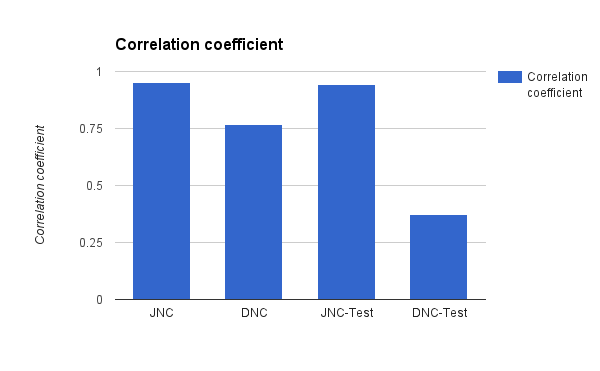
\includegraphics[scale=0.3]{figures/m5Base_1.png} 
\caption{Correlation coefficents for m5Base}
\label{fig:correl_m5base}
\end{figure}

Figure \ref{fig:error_m5base} shows the summary of error tendencies of both games using m5Base. We can see that the MAE and RMSE of JNC is somewhat higher than DNC, but looking into RAE and RRSE, we see that JNC outperforms DNC by a huge difference. The prediction model becomes more reliable than a simple predictor for JNC's case.

\begin{figure}[h!]
\centering
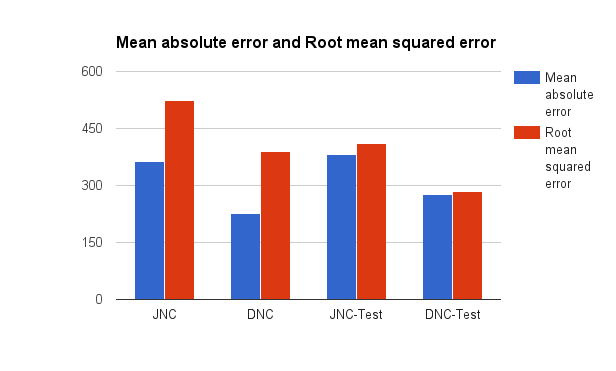
\includegraphics[scale=0.3]{figures/m5Base_2.png} 
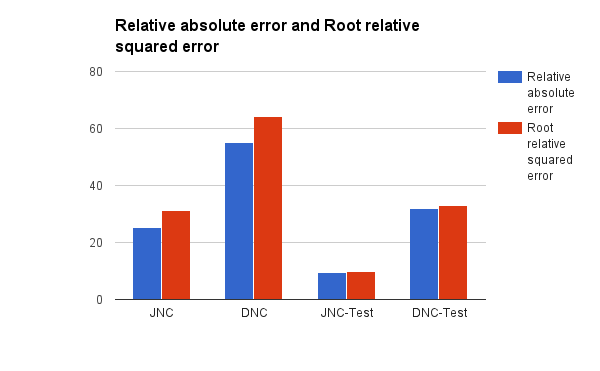
\includegraphics[scale=0.3]{figures/m5Base_3.png} 
\caption{Error tendencies for m5Base}
\label{fig:error_m5base}
\end{figure}

\subsection{REPTree}
We applied REPTree induction for JNC and DNC as it builds a regression tree that is also suitable for real world use. Examining the results, it did not perform on par with the outcome of M5Base. However, the outcome of this learning algorithm  has comparable results than any other learning algorithms we choose. We therefore, mention the results of the model. Fewer features were deemed significant by our feature selection method in REPTree as seen in Table \ref{table:reptree_features}.

\begin{table}[h]
\centering
\caption{Selected features for REPTree}
\label{table:reptree_features}
\begin{tabular}{|c|c|c|}
\hline 
 & Jungle Cubes & Dragon Cubes\\ 
\hline 
Features & Cohort Size & CrashesANRDay1 
\\& DailyAverageRating & LevelFailedEvents 
\\& LevelFailedEvents & Sessions
\\& MKTExpenses & MKTExpenses
\\& MedianSessionSeconds &  
\\& MKTExpenses &  
\\ 
\hline 
\end{tabular}
\end{table}

Table \ref{table:summary_results} shows the summary of metrics for JNC and DNC. Figure \ref{fig:correl_reptree} and Figure \ref{fig:error_reptree} shows the graph of JNC and DNC's correlation coefficients and error tendencies respectively. Notice that JNC and DNC's results on cross-validation procedure did not really differ from the results using m5Base. However, attempting to apply this to our provided test set, we observed that values vary greatly.

\begin{figure}[h]
\centering
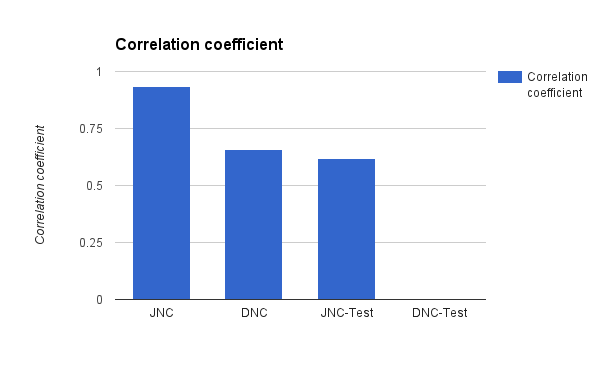
\includegraphics[scale=0.3]{figures/REPTree_1.png} 
\caption{Correlation coefficents for REPTree}
\label{fig:correl_reptree}
\end{figure}

\begin{figure}[h]
\centering
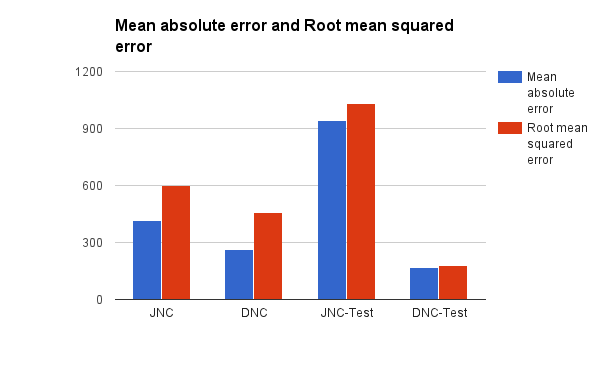
\includegraphics[scale=0.3]{figures/REPTree_2.png} 
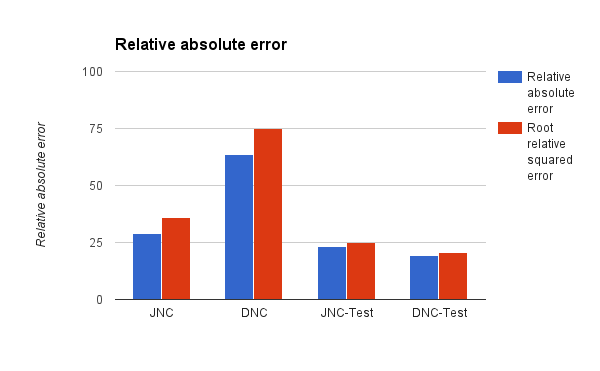
\includegraphics[scale=0.3]{figures/REPTree_3.png} 
\caption{Error tendencies for REPTree}
\label{fig:error_reptree}
\end{figure}

Notice that on \textit{JNC-Test} tab, the error measures has significantly increased compared to m5Base. On the other hand, result in \textbf{DNC-Test} tab indicates that this learning algorithm faired better than m5Base when applied to practical use. However, we cannot fully recommend using REPTree for practical use since the correlation coefficient is zero. There is no real pattern between variables that affect \textbf{DAU-Day7} and may not fully predict \textbf{DAU-Day7} on various events.

\subsection{Multilayer Perceptron}
We attempted to use artificial neural network using Multilayer Perceptron as learning algorithm for predicting \textbf{DAU-Day7}; on the impression that this learning algorithm is flexible and has various parameters involved that we can continuously adjust to improve the accuracy of the model. In this subsection, we discuss briefly how we adjust the settings to generate the optimal network.

Table \ref{table:m5base_features} shows the selected features for multilayer perceptron using our method specified earlier in this paper.

\begin{table}[h]
\centering
\caption{Selected features for Multilayer Perceptron}
\label{table:mp_features}
\begin{tabular}{|c|c|c|}
\hline 
 & Jungle Cubes & Dragon Cubes\\ 
\hline 
Features & Cohort Size & Cohort Size 
\\& MKTExpenses & MKTExpenses 
\\& TotalPurchases &
\\& MedianSessionSeconds &
\\& AvgSessionSeconds &  
\\ 
\hline 
\end{tabular}
\end{table}

We found that the number of hidden layers appropriate for this experiment is the total number of attributes and classes of our dataset\footnote{Actual count from best results has 6 hidden layers. Tally is retrieved after selecting features}. We relied on acceptable training time to modify the learning rate and the total number of epochs. Using the default values provided did not yield acceptable results. Modifying these said parameters\footnote{Learning rate is set to 0.001, number of epochs set to 5000.} noticeably increased the accuracy of the model that is comparable for this study.

Using cross-validation procedure, it can be observed that multilayer perceptron performed acceptably for JNC while DNC did not. The error measures for DNC for multilayer perceptron is the highest among the three numeric prediction models presented.

Applying multilayer perceptron on our test set, observe that JNC have a very low correlation coefficient this time, which is very different from the outcome of REPTree and m5Base. Notice that the MAE and RMSE have significantly increased which makes multilayer perceptron less than ideal for practical use in JNC.

Using multilayer perceptron for DNC, we can observe that the results from the test set closely resemble results from the cross-validation tests in m5Base. The RAE and RRSE is more than 50\% which may indicate that using multilayer perceptron is only halfway better than a simple predictor. 

Table \ref{table:summary_results} shows the summary of the metrics using multilayer perceptron. Figure \ref{fig:correl_mp} and Figure \ref{fig:error_mp} shows the graph for the correlation coefficient and error metrics respectively.

\begin{figure}[h]
\centering
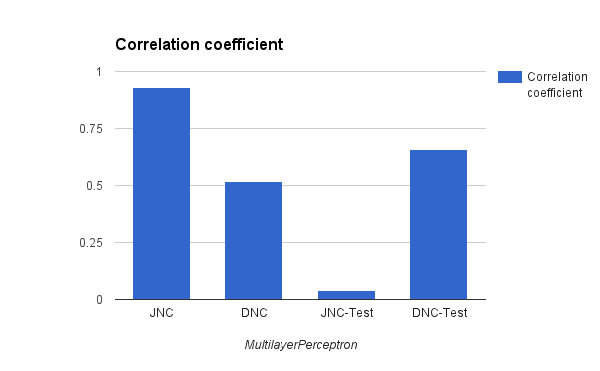
\includegraphics[scale=0.3]{figures/MP_1.png} 
\caption{Correlation coefficents for Multilayer Perceptron}
\label{fig:correl_mp}
\end{figure}

\begin{figure}[h]
\centering
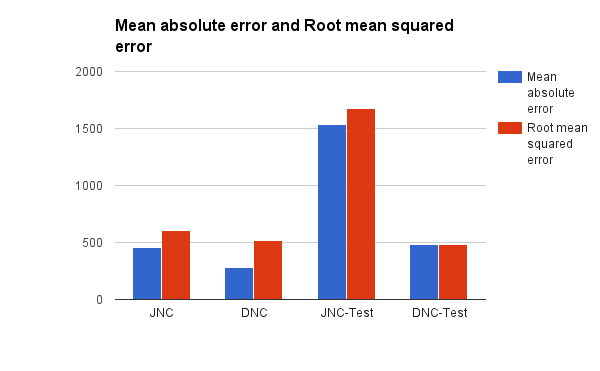
\includegraphics[scale=0.3]{figures/MP_2.png} 
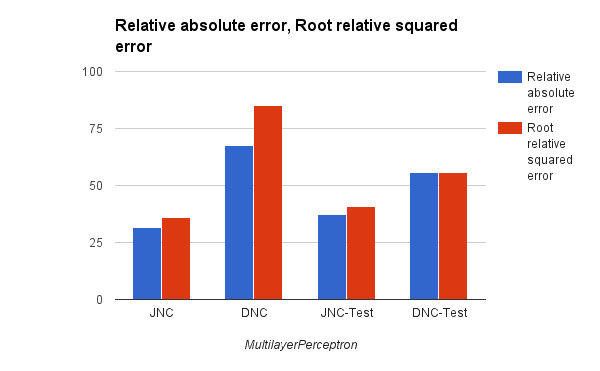
\includegraphics[scale=0.3]{figures/MP_3.png} 
\caption{Error tendencies for Multilayer Perceptron}
\label{fig:error_mp}
\end{figure}

\subsection{Decision-tree induction}
Using our nominal datasets for JNC and DNC, we explored how decision-tree induction will perform\footnote{Using J48 in WEKA}. 

For the case of JNC, we concluded that 5 bins performed best across different test cases for discretization. Using 5 bins, we performed linear forward selection, which is exclusive for JNC and J48 experiment. Using this exclusive feature selection scheme, we managed to slightly have a better accuracy for this test. Our results for JNC on this type of learning algorithm indicates that it does not perform better than using learning algorithms for numeric predictions. For the case of DNC, we notice that using this scheme has resulted into more weight being put on the 1st bin (around 92\%), which made the discretized dataset severely biased. To counter this outcome, we used equal-frequency binning such that using 5 bins, the distribution of weight is even. Table \ref{table:j48_features} shows the features selected for both games using decision-tree induction.

\begin{table*}[h]
\centering
\caption{Summary of results using decision-tree induction}
\label{table:j48_summary_results}
\begin{tabular}{|c|c|c|c|c|}
\hline 
Metrics & JNC & DNC & JNC-Test & DNC-Test \\ 
\hline 
Correctly Classified Instances  & 74.8201\% & 72.8\%  & 92.8571\%  & 100.0\%\\
Incorrectly Classified Instances & 25.1799\% & 27.2\% & 7.1429\% & 0.0\%\\
Kappa statistic & 0.6608 & 0.63 & 0.4717 & 1.000 \\
F-measure & 0.730 & 0.723 & 0.945 & 1.000 \\
Total Number of Instances & 250 & 250 & 28 & 28
\\
\hline 
\end{tabular}
\end{table*}

\begin{table}[h]
\centering
\caption{Selected features for J48}
\label{table:j48_features}
\begin{tabular}{|c|c|c|}
\hline 
 & Jungle Cubes & Dragon Cubes\\ 
\hline 
Features & Cohort Size & Day 1 
\\& LevelPlayedEvents & LevelFailedEvents
\\& Sessions & LevelSuccessEvents 
\\& MKTExpenses & Sessions 
\\& MedianSessionSeconds &MKTExpenses
\\&  &AvgSessionSeconds\\ 
\hline 
\end{tabular}
\end{table}

Referring to Table \ref{table:j48_summary_results}, we can observe that for both JNC and DNC, the overall accuracy of the model does not really differ. While the discretization is different for both games, the overall accuracy are almost similar. Applying the model to our test set, around 7\% of the data in JNC were misclassified while DNC's test set achieved a 100.0\% correctly classification.

For the case of JNC, observing the kappa statistic is only 0.6608 using cross-validation and only 0.4717 on its test set. F-measure is 0.730 and 0.945, using cross-validation and test set respectively. The kappa statistic is lower on the test set which makes the model questionable. With this outcome, we deduce that our test set might not be enough to further recommend using J48 model for actual use. We noticed that our test set do not cover all ranges for \textbf{DAU-Day7}.

This goes the same for DNC but more extreme. The kappa statistic and F-measure are actually \textbf{misleading}. Since there is not much user activity and support for DNC\footnote{Major development for DNC has stopped according to Playlab Inc. and no further acquisition campaigns are implemented when this study was conducted.}, it follows that there will be a low amount of daily active users. On this given circumstance, our model predicted 100\% of such instances in the test set. We can only prove that the model successfully captures this kind of scenario but not on cases where the \textbf{DAU-Day7} is higher.

\subsection{Observations and Recommendations}
We observed that according to our results, accuracies and features selected are different from each learning algorithm. Out of the three learning algorithms proposed, it seems that using m5Base as the prediction model yields the best possible outcome for both games. It favors more for JNC as the dataset being presented has very high correlation coefficient for \textbf{DAU-Day7} unlike DNC.

While REPTree yields the lowest error rate when applied to DNC's test set, we do not recommend using REPTree for long-term use. The current situation of DNC in the gaming market has low acquisition rate, meaning that only a small amount of users get to download the game on a daily basis \footnote{We based this observation from our gathered test set and also observed its trend on Google Play Store.}. Furthermore, marketing expenses for DNC has stopped which may explain the low acquisition rate. This kind of scenario best fit the REPTree prediction model but somehow may not properly predict major changes in user acquisition. We therefore see m5Base as more fitting to consider the scenario where marketing expenses will increase, sudden change in session length or increase of user activity via triggering our custom events.

While multilayer perceptron appear flexible, we do not recommend using multilayer perceptron as prediction model for both games. First, the dataset of both games are small-scale. We therefore need more data to see any clear observations that multilayer perceptron performs acceptably. Training time of the model also consumes more time and CPU performance than the other learning algorithms we've presented, which m5Base and REPTree performed better than multilayer perceptron. Notice that multilayer perceptron performed acceptably on cross-validation method but performed worse when applied to practical use (using test set).

For the case of decision trees, we aim to provide this as a supplement alongside with the preferred prediction model. This works best with using M5Base as both of them are structured as trees. One could use M5Base to determine the regression formula and use the decision tree model to approximate \textbf{DAU-Day7} as additional clarification. Such cases wherein the prediction of M5Base agrees with the result of the decision tree model will make business decisions more reliable. However, DNC's case do not fully capture most of the cases using the decision tree model.

Out of all the learning algorithms used, we see that JNC yields acceptable results. It has low error rates and high correlation coefficient for most tests we've performed. This may justify the success of JNC in the commercial gaming market as we therefore see a trend in the data by just observing the correlation values. However, we do not justify that such trends contribute to the overall increase in daily active users. m5Base yields the highest correlation coefficient across our JNC tests and also produced low error rates. Using the model for practical use, we see that while there is little difference in MAE and RMSE, the RAE and RRSE of JNC yields only 9\%. This makes it suitable for real world use.